\documentclass[twoside]{book}

% Packages required by doxygen
\usepackage{calc}
\usepackage{doxygen}
\usepackage{graphicx}
\usepackage[utf8]{inputenc}
\usepackage{makeidx}
\usepackage{multicol}
\usepackage{multirow}
\usepackage{textcomp}
\usepackage[table]{xcolor}

% Font selection
\usepackage[T1]{fontenc}
\usepackage{mathptmx}
\usepackage[scaled=.90]{helvet}
\usepackage{courier}
\usepackage{amssymb}
\usepackage{sectsty}
\renewcommand{\familydefault}{\sfdefault}
\allsectionsfont{%
  \fontseries{bc}\selectfont%
  \color{darkgray}%
}
\renewcommand{\DoxyLabelFont}{%
  \fontseries{bc}\selectfont%
  \color{darkgray}%
}

% Page & text layout
\usepackage{geometry}
\geometry{%
  a4paper,%
  top=2.5cm,%
  bottom=2.5cm,%
  left=2.5cm,%
  right=2.5cm%
}
\tolerance=750
\hfuzz=15pt
\hbadness=750
\setlength{\emergencystretch}{15pt}
\setlength{\parindent}{0cm}
\setlength{\parskip}{0.2cm}
\makeatletter
\renewcommand{\paragraph}{%
  \@startsection{paragraph}{4}{0ex}{-1.0ex}{1.0ex}{%
    \normalfont\normalsize\bfseries\SS@parafont%
  }%
}
\renewcommand{\subparagraph}{%
  \@startsection{subparagraph}{5}{0ex}{-1.0ex}{1.0ex}{%
    \normalfont\normalsize\bfseries\SS@subparafont%
  }%
}
\makeatother

% Headers & footers
\usepackage{fancyhdr}
\pagestyle{fancyplain}
\fancyhead[LE]{\fancyplain{}{\bfseries\thepage}}
\fancyhead[CE]{\fancyplain{}{}}
\fancyhead[RE]{\fancyplain{}{\bfseries\leftmark}}
\fancyhead[LO]{\fancyplain{}{\bfseries\rightmark}}
\fancyhead[CO]{\fancyplain{}{}}
\fancyhead[RO]{\fancyplain{}{\bfseries\thepage}}
\fancyfoot[LE]{\fancyplain{}{}}
\fancyfoot[CE]{\fancyplain{}{}}
\fancyfoot[RE]{\fancyplain{}{\bfseries\scriptsize Generated on Mon Nov 25 2013 17\-:50\-:39 for Blackjack -\/ Client by Doxygen }}
\fancyfoot[LO]{\fancyplain{}{\bfseries\scriptsize Generated on Mon Nov 25 2013 17\-:50\-:39 for Blackjack -\/ Client by Doxygen }}
\fancyfoot[CO]{\fancyplain{}{}}
\fancyfoot[RO]{\fancyplain{}{}}
\renewcommand{\footrulewidth}{0.4pt}
\renewcommand{\chaptermark}[1]{%
  \markboth{#1}{}%
}
\renewcommand{\sectionmark}[1]{%
  \markright{\thesection\ #1}%
}

% Indices & bibliography
\usepackage{natbib}
\usepackage[titles]{tocloft}
\setcounter{tocdepth}{3}
\setcounter{secnumdepth}{5}
\makeindex

% Hyperlinks (required, but should be loaded last)
\usepackage{ifpdf}
\ifpdf
  \usepackage[pdftex,pagebackref=true]{hyperref}
\else
  \usepackage[ps2pdf,pagebackref=true]{hyperref}
\fi
\hypersetup{%
  colorlinks=true,%
  linkcolor=blue,%
  citecolor=blue,%
  unicode%
}

% Custom commands
\newcommand{\clearemptydoublepage}{%
  \newpage{\pagestyle{empty}\cleardoublepage}%
}


%===== C O N T E N T S =====

\begin{document}

% Titlepage & ToC
\hypersetup{pageanchor=false}
\pagenumbering{roman}
\begin{titlepage}
\vspace*{7cm}
\begin{center}%
{\Large Blackjack -\/ Client \\[1ex]\large Version 1 -\/ \hyperlink{class_client}{Client} }\\
\vspace*{1cm}
{\large Generated by Doxygen 1.8.5}\\
\vspace*{0.5cm}
{\small Mon Nov 25 2013 17:50:39}\\
\end{center}
\end{titlepage}
\clearemptydoublepage
\tableofcontents
\clearemptydoublepage
\pagenumbering{arabic}
\hypersetup{pageanchor=true}

%--- Begin generated contents ---
\chapter{Hierarchical Index}
\section{Class Hierarchy}
This inheritance list is sorted roughly, but not completely, alphabetically\-:\begin{DoxyCompactList}
\item \contentsline{section}{Card}{\pageref{class_card}}{}
\item \contentsline{section}{Card\-Node$<$ D\-T $>$}{\pageref{struct_card_node}}{}
\item \contentsline{section}{Card\-Node$<$ Card $>$}{\pageref{struct_card_node}}{}
\item \contentsline{section}{Hand$<$ D\-T $>$}{\pageref{class_hand}}{}
\item \contentsline{section}{Hand$<$ Card $>$}{\pageref{class_hand}}{}
\item Q\-Frame\begin{DoxyCompactList}
\item \contentsline{section}{Blackjack}{\pageref{class_blackjack}}{}
\end{DoxyCompactList}
\item Q\-Tcp\-Socket\begin{DoxyCompactList}
\item \contentsline{section}{Client}{\pageref{class_client}}{}
\end{DoxyCompactList}
\item Q\-Widget\begin{DoxyCompactList}
\item \contentsline{section}{Blackjack\-Table}{\pageref{class_blackjack_table}}{}
\item \contentsline{section}{Cards\-Set}{\pageref{class_cards_set}}{}
\end{DoxyCompactList}
\item \contentsline{section}{Stack$<$ D\-T $>$}{\pageref{class_stack}}{}
\item \contentsline{section}{Stack$<$ Card $>$}{\pageref{class_stack}}{}
\begin{DoxyCompactList}
\item \contentsline{section}{Deck}{\pageref{class_deck}}{}
\end{DoxyCompactList}
\end{DoxyCompactList}

\chapter{Class Index}
\section{Class List}
Here are the classes, structs, unions and interfaces with brief descriptions\-:\begin{DoxyCompactList}
\item\contentsline{section}{\hyperlink{class_blackjack}{Blackjack} }{\pageref{class_blackjack}}{}
\item\contentsline{section}{\hyperlink{class_blackjack_table}{Blackjack\-Table} }{\pageref{class_blackjack_table}}{}
\item\contentsline{section}{\hyperlink{class_card}{Card} }{\pageref{class_card}}{}
\item\contentsline{section}{\hyperlink{struct_card_node}{Card\-Node$<$ D\-T $>$} }{\pageref{struct_card_node}}{}
\item\contentsline{section}{\hyperlink{class_cards_set}{Cards\-Set} }{\pageref{class_cards_set}}{}
\item\contentsline{section}{\hyperlink{class_client}{Client} }{\pageref{class_client}}{}
\item\contentsline{section}{\hyperlink{class_deck}{Deck} }{\pageref{class_deck}}{}
\item\contentsline{section}{\hyperlink{class_hand}{Hand$<$ D\-T $>$} }{\pageref{class_hand}}{}
\item\contentsline{section}{\hyperlink{class_stack}{Stack$<$ D\-T $>$} }{\pageref{class_stack}}{}
\end{DoxyCompactList}

\chapter{Class Documentation}
\hypertarget{class_blackjack}{\section{Blackjack Class Reference}
\label{class_blackjack}\index{Blackjack@{Blackjack}}
}


{\ttfamily \#include $<$Blackjack.\-h$>$}

Inheritance diagram for Blackjack\-:\begin{figure}[H]
\begin{center}
\leavevmode
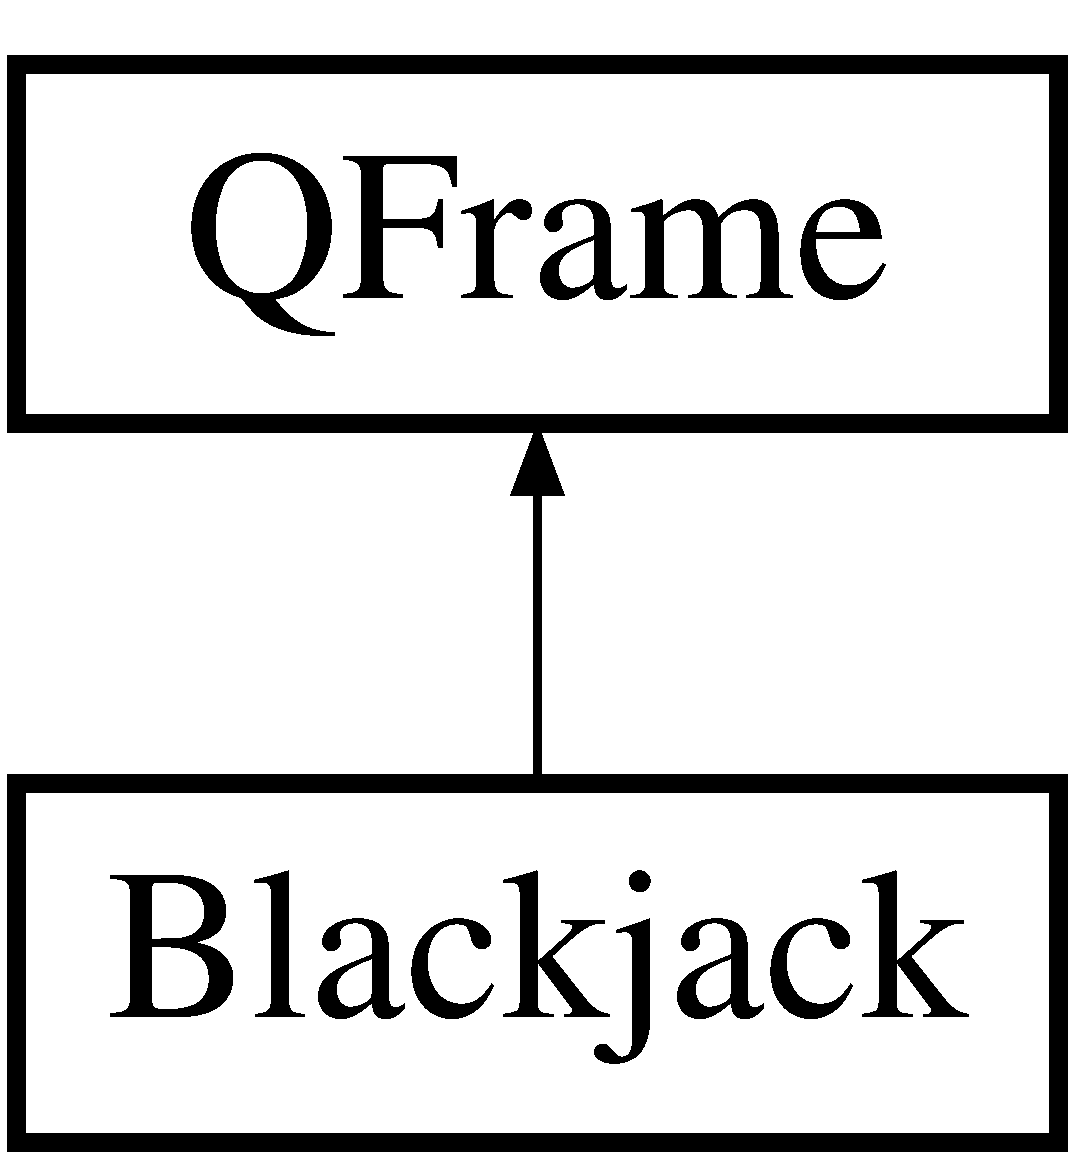
\includegraphics[height=2.000000cm]{class_blackjack}
\end{center}
\end{figure}
\subsection*{Public Member Functions}
\begin{DoxyCompactItemize}
\item 
\hyperlink{class_blackjack_acaeabe885d4c2750b5069e070cb5f84c}{Blackjack} (Q\-Frame $\ast$parent=0)
\begin{DoxyCompactList}\small\item\em Constructor to pull in the Q\-Widget$\ast$ parent. \end{DoxyCompactList}\end{DoxyCompactItemize}


\subsection{Detailed Description}
This header class provides some of the core implementations for the entire game. We hold private slots to many of the most important things of the game, things such as connecting the client, sending a chat message, updating the score table, error logging, and even logging out. In addition to this, this class holds the pointers to various G\-U\-I elements. 

\subsection{Constructor \& Destructor Documentation}
\hypertarget{class_blackjack_acaeabe885d4c2750b5069e070cb5f84c}{\index{Blackjack@{Blackjack}!Blackjack@{Blackjack}}
\index{Blackjack@{Blackjack}!Blackjack@{Blackjack}}
\subsubsection[{Blackjack}]{\setlength{\rightskip}{0pt plus 5cm}Blackjack\-::\-Blackjack (
\begin{DoxyParamCaption}
\item[{Q\-Frame $\ast$}]{parent = {\ttfamily 0}}
\end{DoxyParamCaption}
)}}\label{class_blackjack_acaeabe885d4c2750b5069e070cb5f84c}


Constructor to pull in the Q\-Widget$\ast$ parent. 

Basically let's just pull in the constructor to stop any errors across the board. 
\begin{DoxyParams}{Parameters}
{\em parent} & is basically a var to the Q\-Widget$\ast$ pointer\\
\hline
\end{DoxyParams}
Inst the class and make sure that the frame and stylesheet with the background image is set perfectly. 
\begin{DoxyParams}{Parameters}
{\em parent} & simple Q\-Frame to load our fixed sized loading screen with the pre-\/defined background. \\
\hline
\end{DoxyParams}


The documentation for this class was generated from the following files\-:\begin{DoxyCompactItemize}
\item 
Blackjack.\-h\item 
Blackjack.\-cpp\end{DoxyCompactItemize}

\hypertarget{class_blackjack_table}{\section{Blackjack\-Table Class Reference}
\label{class_blackjack_table}\index{Blackjack\-Table@{Blackjack\-Table}}
}


{\ttfamily \#include $<$Blackjack\-Table.\-h$>$}

Inheritance diagram for Blackjack\-Table\-:\begin{figure}[H]
\begin{center}
\leavevmode
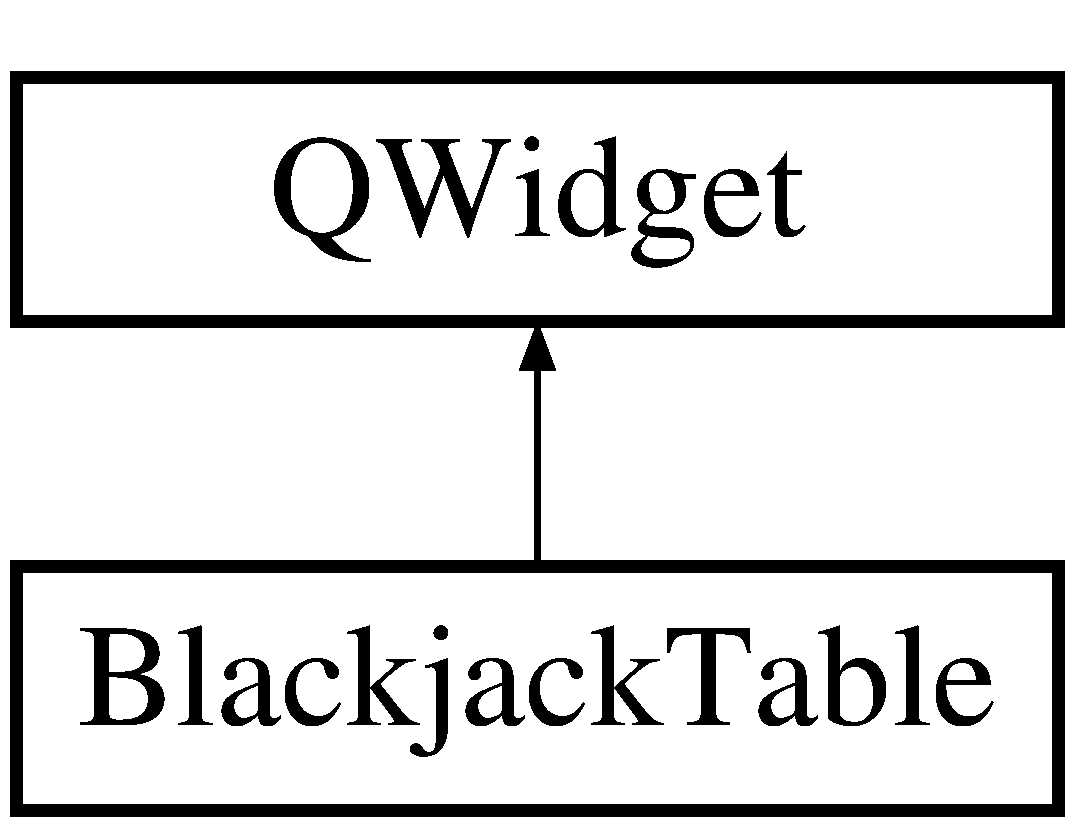
\includegraphics[height=2.000000cm]{class_blackjack_table}
\end{center}
\end{figure}
\subsection*{Signals}
\begin{DoxyCompactItemize}
\item 
void \hyperlink{class_blackjack_table_a54a84c3cf0b00d6b6752ea492cda19a4}{Game\-Finished} (bool user\-Win)
\end{DoxyCompactItemize}
\subsection*{Public Member Functions}
\begin{DoxyCompactItemize}
\item 
\hyperlink{class_blackjack_table_a3b71f8e7d2458679452339977c4b3509}{Blackjack\-Table} (Q\-Widget $\ast$parent=0)
\end{DoxyCompactItemize}


\subsection{Detailed Description}
This class (header) manages the \hyperlink{class_blackjack}{Blackjack} table. Things such as the hit, stand and new game slots are managed from this class. In addition to this we also have the game finished signal in this class. Giving the signal to the slot that controls the game finished allows us to finish the game. 

\subsection{Constructor \& Destructor Documentation}
\hypertarget{class_blackjack_table_a3b71f8e7d2458679452339977c4b3509}{\index{Blackjack\-Table@{Blackjack\-Table}!Blackjack\-Table@{Blackjack\-Table}}
\index{Blackjack\-Table@{Blackjack\-Table}!BlackjackTable@{Blackjack\-Table}}
\subsubsection[{Blackjack\-Table}]{\setlength{\rightskip}{0pt plus 5cm}Blackjack\-Table\-::\-Blackjack\-Table (
\begin{DoxyParamCaption}
\item[{Q\-Widget $\ast$}]{parent = {\ttfamily 0}}
\end{DoxyParamCaption}
)}}\label{class_blackjack_table_a3b71f8e7d2458679452339977c4b3509}
\hyperlink{class_blackjack_table}{Blackjack\-Table} setup that we use to setup all the buttons and grid layouts. 
\begin{DoxyParams}{Parameters}
{\em parent} & basically just to inherit and grab the Widget that we use as the table. \\
\hline
\end{DoxyParams}


\subsection{Member Function Documentation}
\hypertarget{class_blackjack_table_a54a84c3cf0b00d6b6752ea492cda19a4}{\index{Blackjack\-Table@{Blackjack\-Table}!Game\-Finished@{Game\-Finished}}
\index{Game\-Finished@{Game\-Finished}!BlackjackTable@{Blackjack\-Table}}
\subsubsection[{Game\-Finished}]{\setlength{\rightskip}{0pt plus 5cm}void Blackjack\-Table\-::\-Game\-Finished (
\begin{DoxyParamCaption}
\item[{bool}]{user\-Win}
\end{DoxyParamCaption}
)\hspace{0.3cm}{\ttfamily [signal]}}}\label{class_blackjack_table_a54a84c3cf0b00d6b6752ea492cda19a4}
If a message is typed into the line edit box then let's make sure that the message is received to the server and then sent. 
\begin{DoxyParams}{Parameters}
{\em message} & is a Q\-String allowing people to talk over the network.\-This allows us to signal off that the user has won \\
\hline
\end{DoxyParams}


The documentation for this class was generated from the following files\-:\begin{DoxyCompactItemize}
\item 
Blackjack\-Table.\-h\item 
Blackjack\-Table.\-cpp\end{DoxyCompactItemize}

\hypertarget{class_card}{\section{Card Class Reference}
\label{class_card}\index{Card@{Card}}
}


{\ttfamily \#include $<$card.\-h$>$}

\subsection*{Public Member Functions}
\begin{DoxyCompactItemize}
\item 
\hyperlink{class_card_a783f5854cbe8c183ee3d4414c01472c0}{Card} ()
\begin{DoxyCompactList}\small\item\em Constructor for the card, not overloaded just a simple constructor that does nothing. \end{DoxyCompactList}\item 
\hyperlink{class_card_a75f9504162163e35ee8b435418e120c8}{Card} (char s, Q\-String f)
\begin{DoxyCompactList}\small\item\em An overloaded constructor that holds the suit and face of the card. \end{DoxyCompactList}\item 
char \hyperlink{class_card_a9b3bd1aff6901a857f651098e082651d}{get\-\_\-suit} ()
\item 
Q\-String \hyperlink{class_card_afa4d391b07b84127dd5a6fb942dc403c}{get\-\_\-face} ()
\item 
Q\-String \hyperlink{class_card_ab4962a87e9189aa1c197195a346042d2}{get\-\_\-card\-\_\-element} ()
\end{DoxyCompactItemize}


\subsection{Detailed Description}
A lightweight class that allows us to put together the getters of cards so from this class we can get the suit and face cards. Moreover I've put together two private variables for the face and suit cards. 

\subsection{Constructor \& Destructor Documentation}
\hypertarget{class_card_a783f5854cbe8c183ee3d4414c01472c0}{\index{Card@{Card}!Card@{Card}}
\index{Card@{Card}!Card@{Card}}
\subsubsection[{Card}]{\setlength{\rightskip}{0pt plus 5cm}Card\-::\-Card (
\begin{DoxyParamCaption}
{}
\end{DoxyParamCaption}
)}}\label{class_card_a783f5854cbe8c183ee3d4414c01472c0}


Constructor for the card, not overloaded just a simple constructor that does nothing. 

Put together both the front of the card and the suit of the card. We need to know this for later methods and variables.

Very lightweight source file that has mainly getter methods. \hypertarget{class_card_a75f9504162163e35ee8b435418e120c8}{\index{Card@{Card}!Card@{Card}}
\index{Card@{Card}!Card@{Card}}
\subsubsection[{Card}]{\setlength{\rightskip}{0pt plus 5cm}Card\-::\-Card (
\begin{DoxyParamCaption}
\item[{char}]{s, }
\item[{Q\-String}]{f}
\end{DoxyParamCaption}
)}}\label{class_card_a75f9504162163e35ee8b435418e120c8}


An overloaded constructor that holds the suit and face of the card. 

This constructor just basically holds the suit and face of any card. 
\begin{DoxyParams}{Parameters}
{\em s} & is a char for the suit of the card \\
\hline
{\em f} & is a Q\-String for the face of the card\\
\hline
\end{DoxyParams}
Let's get the card value, firstly the suit and secondly we will get the face value of the card. 
\begin{DoxyParams}{Parameters}
{\em s} & the suit card value \\
\hline
{\em f} & the face card value \\
\hline
\end{DoxyParams}


\subsection{Member Function Documentation}
\hypertarget{class_card_ab4962a87e9189aa1c197195a346042d2}{\index{Card@{Card}!get\-\_\-card\-\_\-element@{get\-\_\-card\-\_\-element}}
\index{get\-\_\-card\-\_\-element@{get\-\_\-card\-\_\-element}!Card@{Card}}
\subsubsection[{get\-\_\-card\-\_\-element}]{\setlength{\rightskip}{0pt plus 5cm}Q\-String Card\-::get\-\_\-card\-\_\-element (
\begin{DoxyParamCaption}
{}
\end{DoxyParamCaption}
)}}\label{class_card_ab4962a87e9189aa1c197195a346042d2}
Use a Q\-String to get the card element.

Get the card element, plus the suit. \hypertarget{class_card_afa4d391b07b84127dd5a6fb942dc403c}{\index{Card@{Card}!get\-\_\-face@{get\-\_\-face}}
\index{get\-\_\-face@{get\-\_\-face}!Card@{Card}}
\subsubsection[{get\-\_\-face}]{\setlength{\rightskip}{0pt plus 5cm}Q\-String Card\-::get\-\_\-face (
\begin{DoxyParamCaption}
{}
\end{DoxyParamCaption}
)}}\label{class_card_afa4d391b07b84127dd5a6fb942dc403c}
Get the face value of the card. \hypertarget{class_card_a9b3bd1aff6901a857f651098e082651d}{\index{Card@{Card}!get\-\_\-suit@{get\-\_\-suit}}
\index{get\-\_\-suit@{get\-\_\-suit}!Card@{Card}}
\subsubsection[{get\-\_\-suit}]{\setlength{\rightskip}{0pt plus 5cm}char Card\-::get\-\_\-suit (
\begin{DoxyParamCaption}
{}
\end{DoxyParamCaption}
)}}\label{class_card_a9b3bd1aff6901a857f651098e082651d}
These are getters that allow us to get the suit and face of any particular card that we request.

Get the suit value of the card. 

The documentation for this class was generated from the following files\-:\begin{DoxyCompactItemize}
\item 
card.\-h\item 
card.\-cpp\end{DoxyCompactItemize}

\hypertarget{struct_card_node}{\section{Card\-Node$<$ D\-T $>$ Struct Template Reference}
\label{struct_card_node}\index{Card\-Node$<$ D\-T $>$@{Card\-Node$<$ D\-T $>$}}
}


{\ttfamily \#include $<$stack.\-h$>$}

\subsection*{Public Attributes}
\begin{DoxyCompactItemize}
\item 
\hypertarget{struct_card_node_aaf85d42d125cb3fa84f88683bfbe07bb}{D\-T {\bfseries data}}\label{struct_card_node_aaf85d42d125cb3fa84f88683bfbe07bb}

\item 
\hypertarget{struct_card_node_a213b1d7a1f956945c05c7f4ae1c239c7}{\hyperlink{struct_card_node}{Card\-Node} $\ast$ {\bfseries bottom}}\label{struct_card_node_a213b1d7a1f956945c05c7f4ae1c239c7}

\end{DoxyCompactItemize}


\subsection{Detailed Description}
\subsubsection*{template$<$class D\-T$>$struct Card\-Node$<$ D\-T $>$}

$<$ A template class for the D\-T Struct for the \hyperlink{struct_card_node}{Card\-Node} which goes hand in hand with the stack. We hold the data and the bottom of the stack. 

The documentation for this struct was generated from the following file\-:\begin{DoxyCompactItemize}
\item 
stack.\-h\end{DoxyCompactItemize}

\hypertarget{class_cards_set}{\section{Cards\-Set Class Reference}
\label{class_cards_set}\index{Cards\-Set@{Cards\-Set}}
}


{\ttfamily \#include $<$Cards\-Set.\-h$>$}

Inheritance diagram for Cards\-Set\-:\begin{figure}[H]
\begin{center}
\leavevmode
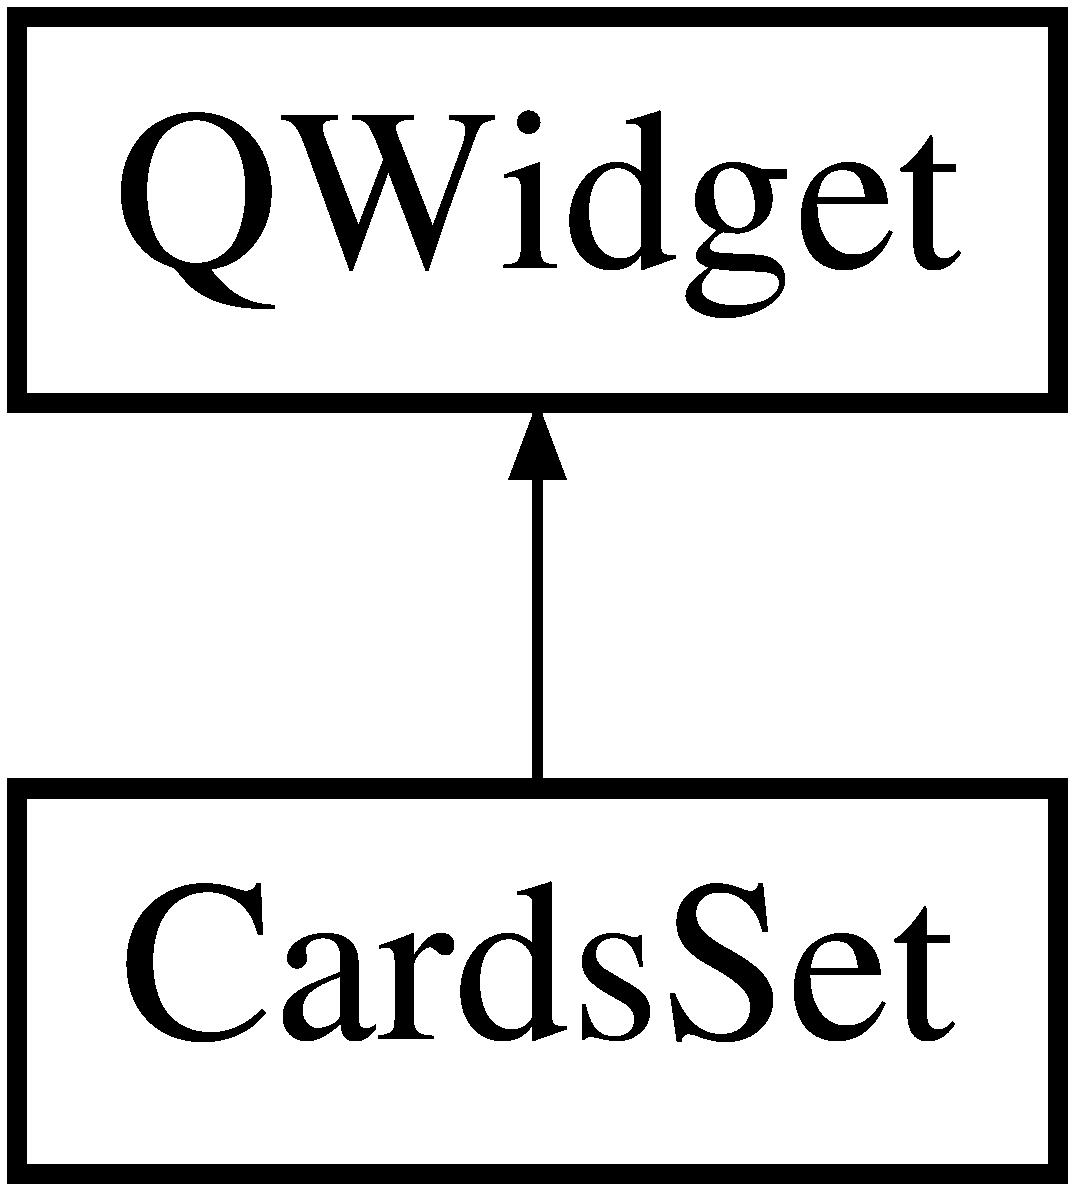
\includegraphics[height=2.000000cm]{class_cards_set}
\end{center}
\end{figure}
\subsection*{Public Member Functions}
\begin{DoxyCompactItemize}
\item 
\hyperlink{class_cards_set_ac2d6c91faf26e135fac8a0b6635807c7}{Cards\-Set} (Q\-Widget $\ast$parent)
\begin{DoxyCompactList}\small\item\em Constructor to pull in the Q\-Widget$\ast$ parent. \end{DoxyCompactList}\item 
void \hyperlink{class_cards_set_a2bda25fc61c9aab36d11c96489cecaa9}{Add\-Card} (Q\-String card\-Name)
\item 
void \hyperlink{class_cards_set_a9fa4f85e786417d6cbe21b2dcf0b09ed}{Clear} ()
\end{DoxyCompactItemize}


\subsection{Detailed Description}
A basic class for the card set, we setup the Q\-Widget and then have a small amount of methods that control adding cards and clearing the deck. In addition to this I've also added a private pointer that points to the layout. 

\subsection{Constructor \& Destructor Documentation}
\hypertarget{class_cards_set_ac2d6c91faf26e135fac8a0b6635807c7}{\index{Cards\-Set@{Cards\-Set}!Cards\-Set@{Cards\-Set}}
\index{Cards\-Set@{Cards\-Set}!CardsSet@{Cards\-Set}}
\subsubsection[{Cards\-Set}]{\setlength{\rightskip}{0pt plus 5cm}Cards\-Set\-::\-Cards\-Set (
\begin{DoxyParamCaption}
\item[{Q\-Widget $\ast$}]{parent}
\end{DoxyParamCaption}
)}}\label{class_cards_set_ac2d6c91faf26e135fac8a0b6635807c7}


Constructor to pull in the Q\-Widget$\ast$ parent. 

We must send the parent for the G\-U\-I to be available. 
\begin{DoxyParams}{Parameters}
{\em parent} & is basically a var to the Q\-Widget$\ast$ pointer.\\
\hline
\end{DoxyParams}
We must make sure that we set the layout and of course pull in the parent widget. 
\begin{DoxyParams}{Parameters}
{\em parent} & is a Q\-Widget pointer to the widget that we use for a layout. \\
\hline
\end{DoxyParams}


\subsection{Member Function Documentation}
\hypertarget{class_cards_set_a2bda25fc61c9aab36d11c96489cecaa9}{\index{Cards\-Set@{Cards\-Set}!Add\-Card@{Add\-Card}}
\index{Add\-Card@{Add\-Card}!CardsSet@{Cards\-Set}}
\subsubsection[{Add\-Card}]{\setlength{\rightskip}{0pt plus 5cm}void Cards\-Set\-::\-Add\-Card (
\begin{DoxyParamCaption}
\item[{Q\-String}]{card\-Name}
\end{DoxyParamCaption}
)}}\label{class_cards_set_a2bda25fc61c9aab36d11c96489cecaa9}
Add to the card set. We use a public method that allows us to the add to the cardset. The card and suit will be determined by another method. 
\begin{DoxyParams}{Parameters}
{\em card\-Name} & a Q\-String for the name of the card.\\
\hline
\end{DoxyParams}
Add a card to the deck and make sure that we keep track of that particular card. 
\begin{DoxyParams}{Parameters}
{\em card\-Name} & we must keep track of this card using a Q\-String. \\
\hline
\end{DoxyParams}
\hypertarget{class_cards_set_a9fa4f85e786417d6cbe21b2dcf0b09ed}{\index{Cards\-Set@{Cards\-Set}!Clear@{Clear}}
\index{Clear@{Clear}!CardsSet@{Cards\-Set}}
\subsubsection[{Clear}]{\setlength{\rightskip}{0pt plus 5cm}void Cards\-Set\-::\-Clear (
\begin{DoxyParamCaption}
{}
\end{DoxyParamCaption}
)}}\label{class_cards_set_a9fa4f85e786417d6cbe21b2dcf0b09ed}
Clear the card set.

Simply clear the card deck and make sure we delete any childen of the cards. 

The documentation for this class was generated from the following files\-:\begin{DoxyCompactItemize}
\item 
Cards\-Set.\-h\item 
Cards\-Set.\-cpp\end{DoxyCompactItemize}

\hypertarget{class_client}{\section{Client Class Reference}
\label{class_client}\index{Client@{Client}}
}


{\ttfamily \#include $<$Client.\-h$>$}

Inheritance diagram for Client\-:\begin{figure}[H]
\begin{center}
\leavevmode
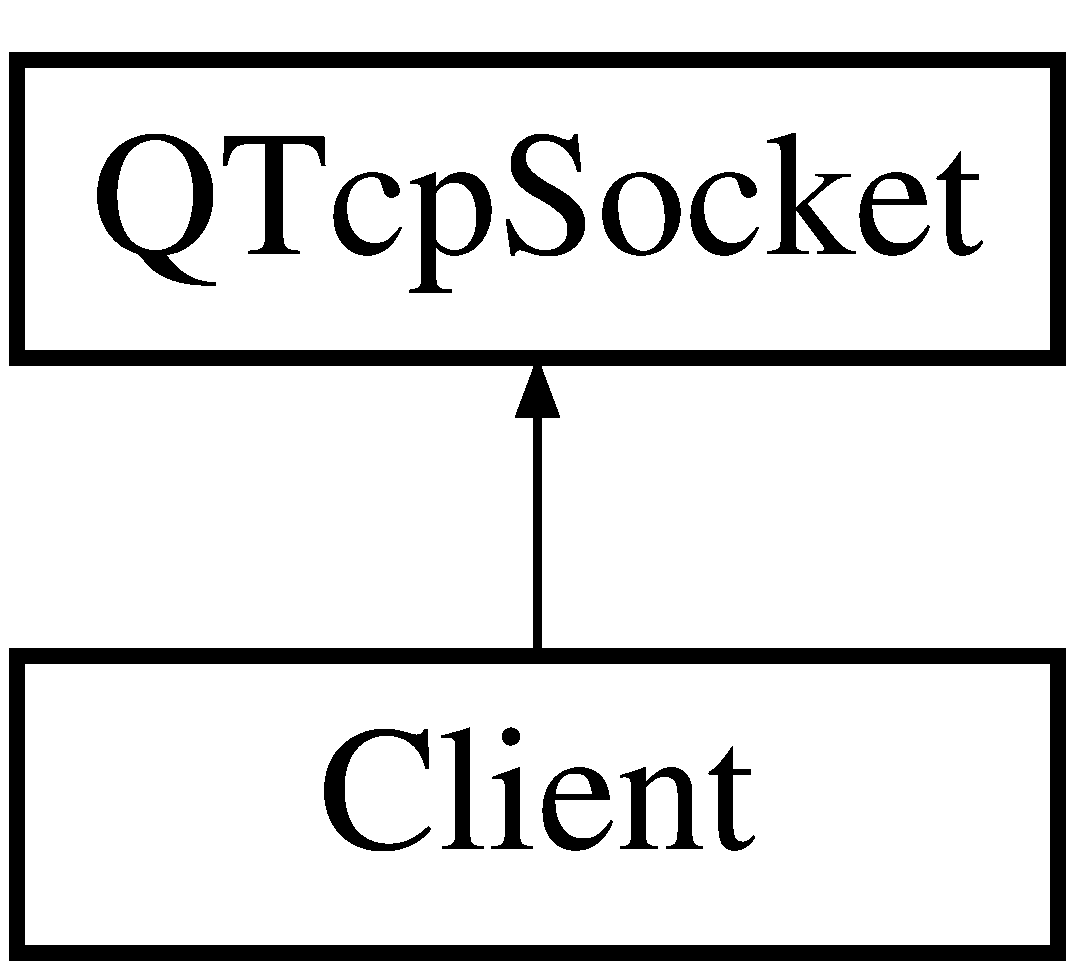
\includegraphics[height=2.000000cm]{class_client}
\end{center}
\end{figure}
\subsection*{Signals}
\begin{DoxyCompactItemize}
\item 
void \hyperlink{class_client_ab7bd1cdd78e0a488cf3f0424ced25c56}{Chat\-Message\-Received} (Q\-String message)
\item 
void \hyperlink{class_client_af5d7d3f9774f38235ebc904e9030ce2e}{Score\-Table\-Results\-Updated} (Q\-String results)
\item 
void \hyperlink{class_client_adc8e44dd81c568518383c6078f3335e5}{Authorization\-Error} ()
\item 
void \hyperlink{class_client_ab933a5ebdc0bcf97ea6c4d8cbb0ffb94}{Log\-Out} ()
\end{DoxyCompactItemize}
\subsection*{Public Member Functions}
\begin{DoxyCompactItemize}
\item 
\hyperlink{class_client_adb0af80eef174ae39ee30dd7565659f8}{Client} (Q\-String username, Q\-Object $\ast$parent=0)
\begin{DoxyCompactList}\small\item\em The client constructor. \end{DoxyCompactList}\item 
bool \hyperlink{class_client_a958fe0409b3ee35c4a84779ec556ad88}{Connect} (unsigned port)
\item 
void \hyperlink{class_client_a57df544a36437362482b5eeab936ea6f}{Send\-Message} (Q\-String message)
\end{DoxyCompactItemize}


\subsection{Detailed Description}
Inherit Q\-Tcp\-Socket as we need it to connect and retrieve information. This class connects up to the Tcp\-Socket and allows us to send signals to the slots that help us connect and disconnect. In addition to this the private slots can connect, disconnect, read messages and show slot errors 

\subsection{Constructor \& Destructor Documentation}
\hypertarget{class_client_adb0af80eef174ae39ee30dd7565659f8}{\index{Client@{Client}!Client@{Client}}
\index{Client@{Client}!Client@{Client}}
\subsubsection[{Client}]{\setlength{\rightskip}{0pt plus 5cm}Client\-::\-Client (
\begin{DoxyParamCaption}
\item[{Q\-String}]{username, }
\item[{Q\-Object $\ast$}]{parent = {\ttfamily 0}}
\end{DoxyParamCaption}
)}}\label{class_client_adb0af80eef174ae39ee30dd7565659f8}


The client constructor. 

We must make sure we construct a client with a username, and if a username is not set we cannot add a client.

Let's connect up the client and set the connections to the server. We also must keep track of the connect and disconnect--esp (signals and slots). 
\begin{DoxyParams}{Parameters}
{\em username} & is a Q\-String to the client's username \\
\hline
{\em parent} & is just basically a pointer to the parent. \\
\hline
\end{DoxyParams}


\subsection{Member Function Documentation}
\hypertarget{class_client_adc8e44dd81c568518383c6078f3335e5}{\index{Client@{Client}!Authorization\-Error@{Authorization\-Error}}
\index{Authorization\-Error@{Authorization\-Error}!Client@{Client}}
\subsubsection[{Authorization\-Error}]{\setlength{\rightskip}{0pt plus 5cm}void Client\-::\-Authorization\-Error (
\begin{DoxyParamCaption}
{}
\end{DoxyParamCaption}
)\hspace{0.3cm}{\ttfamily [signal]}}}\label{class_client_adc8e44dd81c568518383c6078f3335e5}
We must check that there are no errors. If there is an error we signal that there is, and we will then deal with it. \hypertarget{class_client_ab7bd1cdd78e0a488cf3f0424ced25c56}{\index{Client@{Client}!Chat\-Message\-Received@{Chat\-Message\-Received}}
\index{Chat\-Message\-Received@{Chat\-Message\-Received}!Client@{Client}}
\subsubsection[{Chat\-Message\-Received}]{\setlength{\rightskip}{0pt plus 5cm}void Client\-::\-Chat\-Message\-Received (
\begin{DoxyParamCaption}
\item[{Q\-String}]{message}
\end{DoxyParamCaption}
)\hspace{0.3cm}{\ttfamily [signal]}}}\label{class_client_ab7bd1cdd78e0a488cf3f0424ced25c56}
We have to check that the message is in the input box before we can send anything, because we don't want to send bytes down the stream if the line edit is empty. 
\begin{DoxyParams}{Parameters}
{\em message} & is a Q\-String that holds the network'd message. \\
\hline
\end{DoxyParams}
\hypertarget{class_client_a958fe0409b3ee35c4a84779ec556ad88}{\index{Client@{Client}!Connect@{Connect}}
\index{Connect@{Connect}!Client@{Client}}
\subsubsection[{Connect}]{\setlength{\rightskip}{0pt plus 5cm}bool Client\-::\-Connect (
\begin{DoxyParamCaption}
\item[{unsigned}]{port}
\end{DoxyParamCaption}
)}}\label{class_client_a958fe0409b3ee35c4a84779ec556ad88}
We use the bool variable to see if the port is active or not active. By default we will be using the 7777 port as the default because it's far from any normal port, therefore we won't use the same port as something else. 
\begin{DoxyParams}{Parameters}
{\em port} & which is unsigned before we don't know what it is yet.\\
\hline
\end{DoxyParams}
Connect up to the server on a specific port 
\begin{DoxyParams}{Parameters}
{\em port} & is the port we're connect to, generally 7777 \\
\hline
\end{DoxyParams}
\begin{DoxyReturn}{Returns}
the port that we're waiting on to connect 
\end{DoxyReturn}
\hypertarget{class_client_ab933a5ebdc0bcf97ea6c4d8cbb0ffb94}{\index{Client@{Client}!Log\-Out@{Log\-Out}}
\index{Log\-Out@{Log\-Out}!Client@{Client}}
\subsubsection[{Log\-Out}]{\setlength{\rightskip}{0pt plus 5cm}void Client\-::\-Log\-Out (
\begin{DoxyParamCaption}
{}
\end{DoxyParamCaption}
)\hspace{0.3cm}{\ttfamily [signal]}}}\label{class_client_ab933a5ebdc0bcf97ea6c4d8cbb0ffb94}
It's imperative that we have a Log\-Out function so that we can get rid of any connections that might be held up on the server. \hypertarget{class_client_af5d7d3f9774f38235ebc904e9030ce2e}{\index{Client@{Client}!Score\-Table\-Results\-Updated@{Score\-Table\-Results\-Updated}}
\index{Score\-Table\-Results\-Updated@{Score\-Table\-Results\-Updated}!Client@{Client}}
\subsubsection[{Score\-Table\-Results\-Updated}]{\setlength{\rightskip}{0pt plus 5cm}void Client\-::\-Score\-Table\-Results\-Updated (
\begin{DoxyParamCaption}
\item[{Q\-String}]{results}
\end{DoxyParamCaption}
)\hspace{0.3cm}{\ttfamily [signal]}}}\label{class_client_af5d7d3f9774f38235ebc904e9030ce2e}
Update the scores on the score table. This will signal to the method that we have a results update and we must update the table. 
\begin{DoxyParams}{Parameters}
{\em results} & is a Q\-String that holds the data that we cut up. \\
\hline
\end{DoxyParams}
\hypertarget{class_client_a57df544a36437362482b5eeab936ea6f}{\index{Client@{Client}!Send\-Message@{Send\-Message}}
\index{Send\-Message@{Send\-Message}!Client@{Client}}
\subsubsection[{Send\-Message}]{\setlength{\rightskip}{0pt plus 5cm}void Client\-::\-Send\-Message (
\begin{DoxyParamCaption}
\item[{Q\-String}]{message}
\end{DoxyParamCaption}
)}}\label{class_client_a57df544a36437362482b5eeab936ea6f}
Constructor to pull in the Q\-Widget$\ast$ parent 
\begin{DoxyParams}{Parameters}
{\em message} & is basically a Q\-String var to send a message down the network.\\
\hline
\end{DoxyParams}
We use this method as a lower method that uses a bytearray and a datastream. We set the version of the blocks to 16 bytes. 
\begin{DoxyParams}{Parameters}
{\em message} & that we send across the local network. \\
\hline
\end{DoxyParams}


The documentation for this class was generated from the following files\-:\begin{DoxyCompactItemize}
\item 
Client.\-h\item 
Client.\-cpp\end{DoxyCompactItemize}

\hypertarget{class_deck}{\section{Deck Class Reference}
\label{class_deck}\index{Deck@{Deck}}
}


{\ttfamily \#include $<$deck.\-h$>$}

Inheritance diagram for Deck\-:\begin{figure}[H]
\begin{center}
\leavevmode
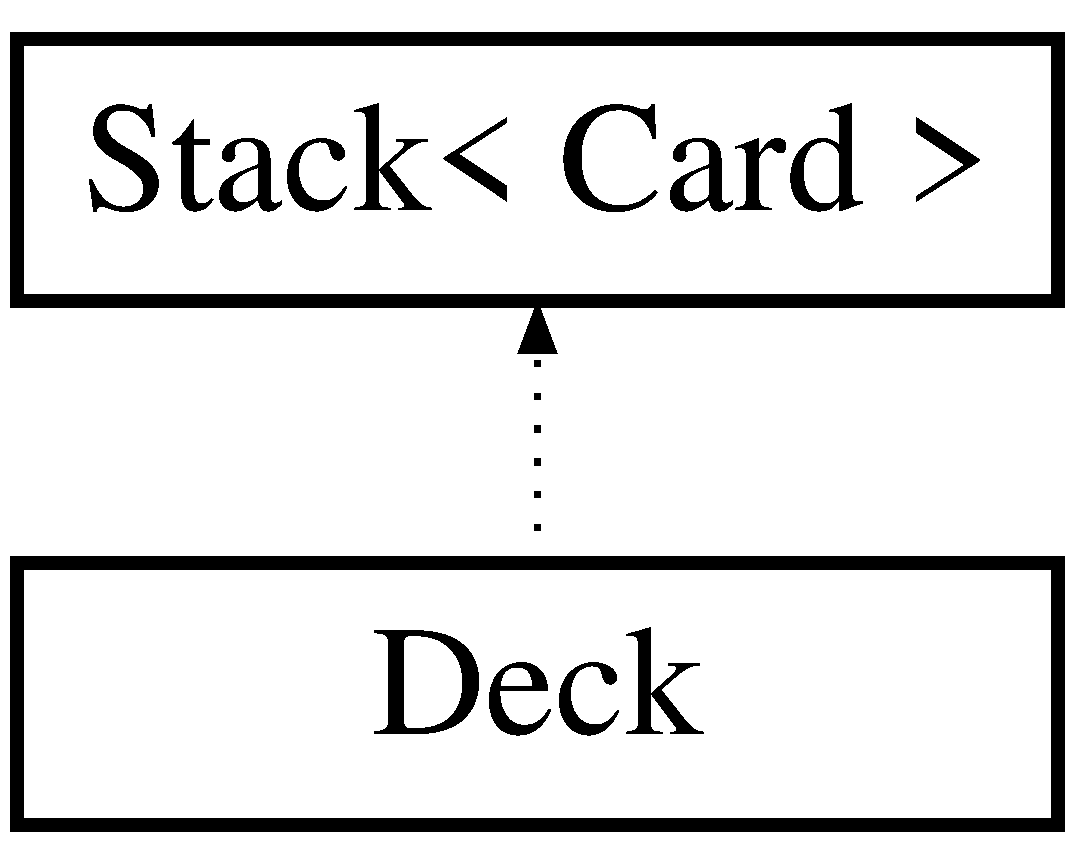
\includegraphics[height=2.000000cm]{class_deck}
\end{center}
\end{figure}
\subsection*{Public Member Functions}
\begin{DoxyCompactItemize}
\item 
\hyperlink{class_deck_a57ae1cb4ac6fd61c249cefb2db85eb99}{Deck} ()
\begin{DoxyCompactList}\small\item\em Constructor for the deck. \end{DoxyCompactList}\item 
void \hyperlink{class_deck_a1036fba7b0c9e1ce8c78aae21a62594c}{get\-Data} ()
\item 
void \hyperlink{class_deck_ad3802b8719178824b95c5cbbca184ea1}{clear\-\_\-deck} ()
\item 
\hyperlink{class_card}{Card} \hyperlink{class_deck_a16604aabf7fc56dd44a72c4e862758cf}{deal} ()
\item 
int \hyperlink{class_deck_a737f7e2a1351f908be1da4d9edcc483b}{get\-\_\-deck\-\_\-size} ()
\end{DoxyCompactItemize}


\subsection{Detailed Description}
This class \hyperlink{class_deck}{Deck} inherits the stack and the card object so that we can keep pushing and popping cards onto the stack. This class holds the data for face cards, suit cards and a vector set to hold the cards. 

\subsection{Constructor \& Destructor Documentation}
\hypertarget{class_deck_a57ae1cb4ac6fd61c249cefb2db85eb99}{\index{Deck@{Deck}!Deck@{Deck}}
\index{Deck@{Deck}!Deck@{Deck}}
\subsubsection[{Deck}]{\setlength{\rightskip}{0pt plus 5cm}Deck\-::\-Deck (
\begin{DoxyParamCaption}
{}
\end{DoxyParamCaption}
)\hspace{0.3cm}{\ttfamily [inline]}}}\label{class_deck_a57ae1cb4ac6fd61c249cefb2db85eb99}


Constructor for the deck. 

Constructor for the \hyperlink{class_deck}{Deck} that holds the stack that holds a card 
\begin{DoxyParams}{Parameters}
{\em \hyperlink{class_card}{Card}} & we must push a card onto the stack \\
\hline
\end{DoxyParams}
We must get the data from the method below that gives us the face and suit of the card.

\subsection{Member Function Documentation}
\hypertarget{class_deck_ad3802b8719178824b95c5cbbca184ea1}{\index{Deck@{Deck}!clear\-\_\-deck@{clear\-\_\-deck}}
\index{clear\-\_\-deck@{clear\-\_\-deck}!Deck@{Deck}}
\subsubsection[{clear\-\_\-deck}]{\setlength{\rightskip}{0pt plus 5cm}void Deck\-::clear\-\_\-deck (
\begin{DoxyParamCaption}
{}
\end{DoxyParamCaption}
)\hspace{0.3cm}{\ttfamily [inline]}}}\label{class_deck_ad3802b8719178824b95c5cbbca184ea1}
Let's clear the deck, using thd \hyperlink{class_stack_acce5debc5c2f8e0cb5238af3d6ddc433}{Deck\-::clear()} method, after that we get new data. \hypertarget{class_deck_a16604aabf7fc56dd44a72c4e862758cf}{\index{Deck@{Deck}!deal@{deal}}
\index{deal@{deal}!Deck@{Deck}}
\subsubsection[{deal}]{\setlength{\rightskip}{0pt plus 5cm}{\bf Card} Deck\-::deal (
\begin{DoxyParamCaption}
{}
\end{DoxyParamCaption}
)\hspace{0.3cm}{\ttfamily [inline]}}}\label{class_deck_a16604aabf7fc56dd44a72c4e862758cf}
Deal the cards and then get the value of the card. Once we've done this we will pop the stack, once that is done, let's return the value. $<$ a \hyperlink{class_card}{Card} class value

$<$ return the value of the card when it's delt \hypertarget{class_deck_a737f7e2a1351f908be1da4d9edcc483b}{\index{Deck@{Deck}!get\-\_\-deck\-\_\-size@{get\-\_\-deck\-\_\-size}}
\index{get\-\_\-deck\-\_\-size@{get\-\_\-deck\-\_\-size}!Deck@{Deck}}
\subsubsection[{get\-\_\-deck\-\_\-size}]{\setlength{\rightskip}{0pt plus 5cm}int Deck\-::get\-\_\-deck\-\_\-size (
\begin{DoxyParamCaption}
{}
\end{DoxyParamCaption}
)\hspace{0.3cm}{\ttfamily [inline]}}}\label{class_deck_a737f7e2a1351f908be1da4d9edcc483b}
Let's get the size of the deck, as we need to know this sometimes. \begin{DoxyReturn}{Returns}
Deck\-::\-Size() this allows us to get the size of the deck. 
\end{DoxyReturn}
\hypertarget{class_deck_a1036fba7b0c9e1ce8c78aae21a62594c}{\index{Deck@{Deck}!get\-Data@{get\-Data}}
\index{get\-Data@{get\-Data}!Deck@{Deck}}
\subsubsection[{get\-Data}]{\setlength{\rightskip}{0pt plus 5cm}void Deck\-::get\-Data (
\begin{DoxyParamCaption}
{}
\end{DoxyParamCaption}
)\hspace{0.3cm}{\ttfamily [inline]}}}\label{class_deck_a1036fba7b0c9e1ce8c78aae21a62594c}
Here we can get the data. Basically the data is the details of the cards, such as the suit of the card and the face of the card. A lot of functionality is implemented within this method. We shuffle the cards in the vectors too, when that's done and a user is playing we push and pop the stack. Face cards Q\-String array that holds the numbers of the cards.

Char suit cards array that holds the chars to the values of the cards.

Vector that holds cards, these cards are passed in as objects.

Vector that holds cards, these cards are iterations--passed in as objects.

$<$ Let's get a random value

Here we are adding the 52 cards to the card\-\_\-vector\-\_\-holder, we do this by passing in the faces and suits.

Let's use a random shuffle starting at the begining of the card\-\_\-vector\-\_\-holder, once we've done that we'll finish up at card\-\_\-vector\-\_\-holder, but at the end.

Let's push the cards onto the stack.

The documentation for this class was generated from the following file\-:\begin{DoxyCompactItemize}
\item 
deck.\-h\end{DoxyCompactItemize}

\hypertarget{class_hand}{\section{Hand$<$ D\-T $>$ Class Template Reference}
\label{class_hand}\index{Hand$<$ D\-T $>$@{Hand$<$ D\-T $>$}}
}


{\ttfamily \#include $<$hand.\-h$>$}

\subsection*{Public Member Functions}
\begin{DoxyCompactItemize}
\item 
\hyperlink{class_hand_ae3cef74a1e4a2cf45d630b347b923eae}{Hand} ()
\begin{DoxyCompactList}\small\item\em The \hyperlink{class_hand}{Hand} Constructor. \end{DoxyCompactList}\item 
\hyperlink{class_hand_a021a43d1a2eff97afed21395e70181e1}{$\sim$\-Hand} ()
\begin{DoxyCompactList}\small\item\em The \hyperlink{class_hand}{Hand} destructor. \end{DoxyCompactList}\item 
bool \hyperlink{class_hand_a912c20114230b88f5e578a899d7e75c6}{add} (D\-T new\-\_\-card)
\item 
void \hyperlink{class_hand_a665d8404a3b51991a0d0a0a3fc4c9a4e}{clear} ()
\item 
int \hyperlink{class_hand_a13520d75c81712f57a18c81322137b72}{value} ()
\item 
int \hyperlink{class_hand_a5e73744dfcbb49d33958702fa6b6da6a}{hand\-\_\-size} ()
\end{DoxyCompactItemize}


\subsection{Detailed Description}
\subsubsection*{template$<$class D\-T$>$class Hand$<$ D\-T $>$}

$<$ A template class for the D\-T This class holds the hand values and what the size of the hand is, what is currently going on within the game and if we need a new hand. We can also get the value of a card here. Moreover we can also get the hand size. 

\subsection{Constructor \& Destructor Documentation}
\hypertarget{class_hand_ae3cef74a1e4a2cf45d630b347b923eae}{\index{Hand@{Hand}!Hand@{Hand}}
\index{Hand@{Hand}!Hand@{Hand}}
\subsubsection[{Hand}]{\setlength{\rightskip}{0pt plus 5cm}template$<$class D\-T$>$ {\bf Hand}$<$ D\-T $>$\-::{\bf Hand} (
\begin{DoxyParamCaption}
{}
\end{DoxyParamCaption}
)\hspace{0.3cm}{\ttfamily [inline]}}}\label{class_hand_ae3cef74a1e4a2cf45d630b347b923eae}


The \hyperlink{class_hand}{Hand} Constructor. 

We call init to make sure we have a game ready to play. \hypertarget{class_hand_a021a43d1a2eff97afed21395e70181e1}{\index{Hand@{Hand}!$\sim$\-Hand@{$\sim$\-Hand}}
\index{$\sim$\-Hand@{$\sim$\-Hand}!Hand@{Hand}}
\subsubsection[{$\sim$\-Hand}]{\setlength{\rightskip}{0pt plus 5cm}template$<$class D\-T$>$ {\bf Hand}$<$ D\-T $>$\-::$\sim${\bf Hand} (
\begin{DoxyParamCaption}
{}
\end{DoxyParamCaption}
)\hspace{0.3cm}{\ttfamily [inline]}}}\label{class_hand_a021a43d1a2eff97afed21395e70181e1}


The \hyperlink{class_hand}{Hand} destructor. 

Destroy the cards and make sure we deconstruct. 

\subsection{Member Function Documentation}
\hypertarget{class_hand_a912c20114230b88f5e578a899d7e75c6}{\index{Hand@{Hand}!add@{add}}
\index{add@{add}!Hand@{Hand}}
\subsubsection[{add}]{\setlength{\rightskip}{0pt plus 5cm}template$<$class D\-T$>$ bool {\bf Hand}$<$ D\-T $>$\-::add (
\begin{DoxyParamCaption}
\item[{D\-T}]{new\-\_\-card}
\end{DoxyParamCaption}
)\hspace{0.3cm}{\ttfamily [inline]}}}\label{class_hand_a912c20114230b88f5e578a899d7e75c6}
Add a new card. \begin{DoxyReturn}{Returns}
true at the end of the method. 
\end{DoxyReturn}
\hypertarget{class_hand_a665d8404a3b51991a0d0a0a3fc4c9a4e}{\index{Hand@{Hand}!clear@{clear}}
\index{clear@{clear}!Hand@{Hand}}
\subsubsection[{clear}]{\setlength{\rightskip}{0pt plus 5cm}template$<$class D\-T$>$ void {\bf Hand}$<$ D\-T $>$\-::clear (
\begin{DoxyParamCaption}
{}
\end{DoxyParamCaption}
)\hspace{0.3cm}{\ttfamily [inline]}}}\label{class_hand_a665d8404a3b51991a0d0a0a3fc4c9a4e}
Clear the cards. \hypertarget{class_hand_a5e73744dfcbb49d33958702fa6b6da6a}{\index{Hand@{Hand}!hand\-\_\-size@{hand\-\_\-size}}
\index{hand\-\_\-size@{hand\-\_\-size}!Hand@{Hand}}
\subsubsection[{hand\-\_\-size}]{\setlength{\rightskip}{0pt plus 5cm}template$<$class D\-T$>$ int {\bf Hand}$<$ D\-T $>$\-::hand\-\_\-size (
\begin{DoxyParamCaption}
{}
\end{DoxyParamCaption}
)\hspace{0.3cm}{\ttfamily [inline]}}}\label{class_hand_a5e73744dfcbb49d33958702fa6b6da6a}
Get the hand size. \begin{DoxyReturn}{Returns}
the hand size (example\-: 21) 
\end{DoxyReturn}
\hypertarget{class_hand_a13520d75c81712f57a18c81322137b72}{\index{Hand@{Hand}!value@{value}}
\index{value@{value}!Hand@{Hand}}
\subsubsection[{value}]{\setlength{\rightskip}{0pt plus 5cm}template$<$class D\-T$>$ int {\bf Hand}$<$ D\-T $>$\-::value (
\begin{DoxyParamCaption}
{}
\end{DoxyParamCaption}
)\hspace{0.3cm}{\ttfamily [inline]}}}\label{class_hand_a13520d75c81712f57a18c81322137b72}
Get the value of the cards. $<$ set card value to zero.

Get value of the cards and the face and suit of the cards.

We have to see what the value of the ace is.

$<$ return the value of the suited card. 

The documentation for this class was generated from the following file\-:\begin{DoxyCompactItemize}
\item 
hand.\-h\end{DoxyCompactItemize}

\hypertarget{class_stack}{\section{Stack$<$ D\-T $>$ Class Template Reference}
\label{class_stack}\index{Stack$<$ D\-T $>$@{Stack$<$ D\-T $>$}}
}


{\ttfamily \#include $<$stack.\-h$>$}

\subsection*{Public Member Functions}
\begin{DoxyCompactItemize}
\item 
\hyperlink{class_stack_ad41e41e610dc6cf9bb229160f5f205d3}{Stack} ()
\begin{DoxyCompactList}\small\item\em The stack constructor. \end{DoxyCompactList}\item 
\hyperlink{class_stack_a72a1b990711e7d12b8fd0804b431ad22}{$\sim$\-Stack} ()
\begin{DoxyCompactList}\small\item\em The stack deconstructor. \end{DoxyCompactList}\item 
int \hyperlink{class_stack_a08eb7cd8ca96965989c17405808b9d42}{size} ()
\item 
bool \hyperlink{class_stack_a37519366e7a3b338bdc278a9c9b8a131}{push} (D\-T new\-\_\-card)
\item 
bool \hyperlink{class_stack_a9f16d1c68cef90bc1859afd6fce88734}{pop} (D\-T \&get\-\_\-card)
\item 
void \hyperlink{class_stack_acce5debc5c2f8e0cb5238af3d6ddc433}{clear} ()
\end{DoxyCompactItemize}


\subsection{Detailed Description}
\subsubsection*{template$<$class D\-T$>$class Stack$<$ D\-T $>$}

$<$ A template class for the D\-T All the cards are stored on the stack, it makes it really easy to control what is going on. We can push and pop of the stack. 

\subsection{Constructor \& Destructor Documentation}
\hypertarget{class_stack_ad41e41e610dc6cf9bb229160f5f205d3}{\index{Stack@{Stack}!Stack@{Stack}}
\index{Stack@{Stack}!Stack@{Stack}}
\subsubsection[{Stack}]{\setlength{\rightskip}{0pt plus 5cm}template$<$class D\-T$>$ {\bf Stack}$<$ D\-T $>$\-::{\bf Stack} (
\begin{DoxyParamCaption}
{}
\end{DoxyParamCaption}
)\hspace{0.3cm}{\ttfamily [inline]}}}\label{class_stack_ad41e41e610dc6cf9bb229160f5f205d3}


The stack constructor. 

We must set the top of the stack to N\-U\-L\-L. The next value is then set to 0. \hypertarget{class_stack_a72a1b990711e7d12b8fd0804b431ad22}{\index{Stack@{Stack}!$\sim$\-Stack@{$\sim$\-Stack}}
\index{$\sim$\-Stack@{$\sim$\-Stack}!Stack@{Stack}}
\subsubsection[{$\sim$\-Stack}]{\setlength{\rightskip}{0pt plus 5cm}template$<$class D\-T$>$ {\bf Stack}$<$ D\-T $>$\-::$\sim${\bf Stack} (
\begin{DoxyParamCaption}
{}
\end{DoxyParamCaption}
)\hspace{0.3cm}{\ttfamily [inline]}}}\label{class_stack_a72a1b990711e7d12b8fd0804b431ad22}


The stack deconstructor. 

We must clear the stack when we deconstruct. 

\subsection{Member Function Documentation}
\hypertarget{class_stack_acce5debc5c2f8e0cb5238af3d6ddc433}{\index{Stack@{Stack}!clear@{clear}}
\index{clear@{clear}!Stack@{Stack}}
\subsubsection[{clear}]{\setlength{\rightskip}{0pt plus 5cm}template$<$class D\-T$>$ void {\bf Stack}$<$ D\-T $>$\-::clear (
\begin{DoxyParamCaption}
{}
\end{DoxyParamCaption}
)\hspace{0.3cm}{\ttfamily [inline]}}}\label{class_stack_acce5debc5c2f8e0cb5238af3d6ddc433}
Clear the stack and remove any node or value. \hypertarget{class_stack_a9f16d1c68cef90bc1859afd6fce88734}{\index{Stack@{Stack}!pop@{pop}}
\index{pop@{pop}!Stack@{Stack}}
\subsubsection[{pop}]{\setlength{\rightskip}{0pt plus 5cm}template$<$class D\-T$>$ bool {\bf Stack}$<$ D\-T $>$\-::pop (
\begin{DoxyParamCaption}
\item[{D\-T \&}]{get\-\_\-card}
\end{DoxyParamCaption}
)\hspace{0.3cm}{\ttfamily [inline]}}}\label{class_stack_a9f16d1c68cef90bc1859afd6fce88734}
Let's pop the top of the stack and get the pointer value of the card. 
\begin{DoxyParams}{Parameters}
{\em \&get\-\_\-card} & address so we can pop it from the stack. \\
\hline
\end{DoxyParams}
\begin{DoxyReturn}{Returns}
true when we have the card. 
\end{DoxyReturn}
\hypertarget{class_stack_a37519366e7a3b338bdc278a9c9b8a131}{\index{Stack@{Stack}!push@{push}}
\index{push@{push}!Stack@{Stack}}
\subsubsection[{push}]{\setlength{\rightskip}{0pt plus 5cm}template$<$class D\-T$>$ bool {\bf Stack}$<$ D\-T $>$\-::push (
\begin{DoxyParamCaption}
\item[{D\-T}]{new\-\_\-card}
\end{DoxyParamCaption}
)\hspace{0.3cm}{\ttfamily [inline]}}}\label{class_stack_a37519366e7a3b338bdc278a9c9b8a131}
Let's push onto the stack. 
\begin{DoxyParams}{Parameters}
{\em new\-\_\-card} & to add to the \hyperlink{struct_card_node}{Card\-Node}. \\
\hline
\end{DoxyParams}
\begin{DoxyReturn}{Returns}
stack size. 
\end{DoxyReturn}
\hypertarget{class_stack_a08eb7cd8ca96965989c17405808b9d42}{\index{Stack@{Stack}!size@{size}}
\index{size@{size}!Stack@{Stack}}
\subsubsection[{size}]{\setlength{\rightskip}{0pt plus 5cm}template$<$class D\-T$>$ int {\bf Stack}$<$ D\-T $>$\-::size (
\begin{DoxyParamCaption}
{}
\end{DoxyParamCaption}
)\hspace{0.3cm}{\ttfamily [inline]}}}\label{class_stack_a08eb7cd8ca96965989c17405808b9d42}
Let's return the size of the stack. \begin{DoxyReturn}{Returns}
stack size. 
\end{DoxyReturn}


The documentation for this class was generated from the following file\-:\begin{DoxyCompactItemize}
\item 
stack.\-h\end{DoxyCompactItemize}

%--- End generated contents ---

% Index
\newpage
\phantomsection
\addcontentsline{toc}{part}{Index}
\printindex

\end{document}
